\section{Results}
In the following section per convention $\lambda$ is the wavelength $d$ is the with of the slit and $z$ is the distance from the screen.\\
As can be seen in figure \ref{fig:single slit interference with 0.04mm width} the theory for a single slit fits the data well however there are
secondary effects easily observable in the tails of the data that per our understanding are partially caused by the non-linearity of the
photomultiplier and photoelectric sensor, such effects were not taken into account when formulating our theory
However the adjustment can be easily accomplished.
\begin{figure}[H]
    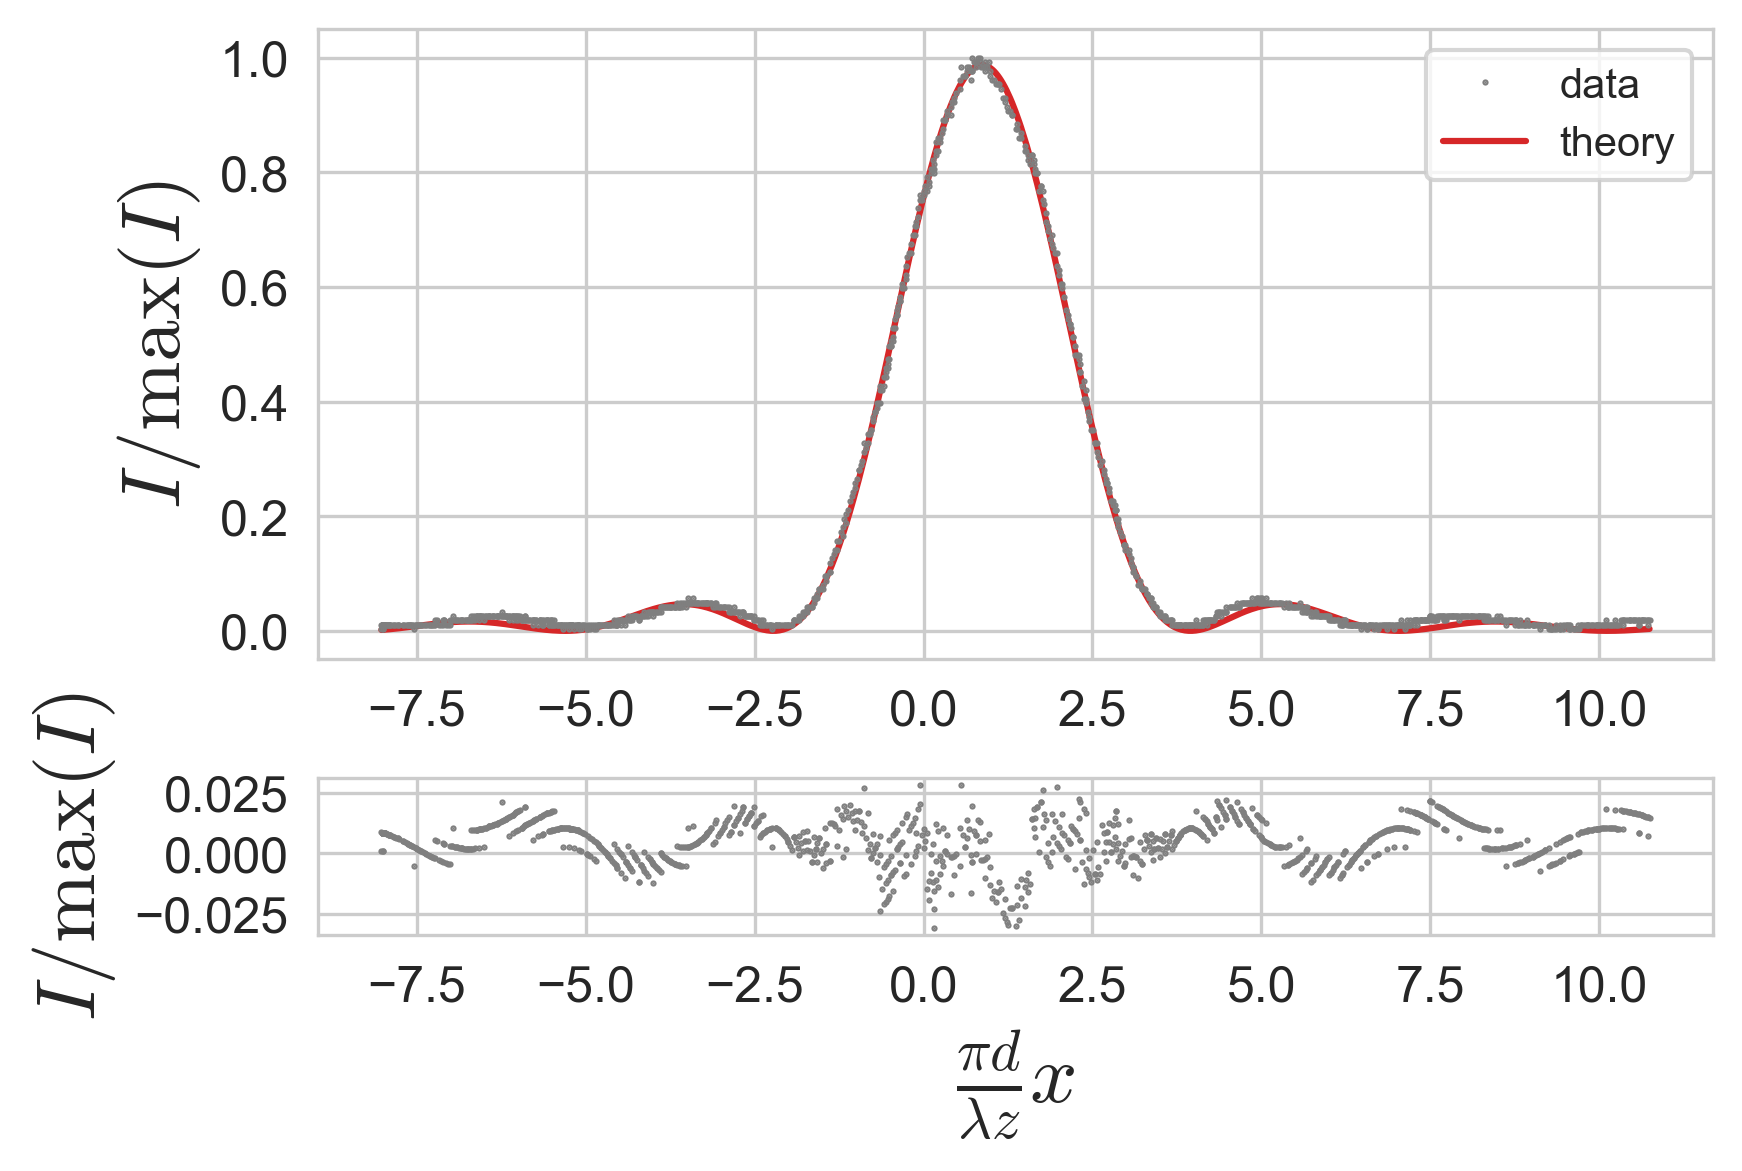
\includegraphics[width=0.9\columnwidth]{figures/single slit interference with 0.04mm width.png}
    \caption{$\lambda$ is the laser wave length $d$ is the width of the slit and $z$ is the distance from the screen}
    \label{fig:single slit interference with 0.04mm width}
\end{figure}
\begin{figure}[H]
	\centering
	\begin{subfigure}{0.5\columnwidth}
		\centering
		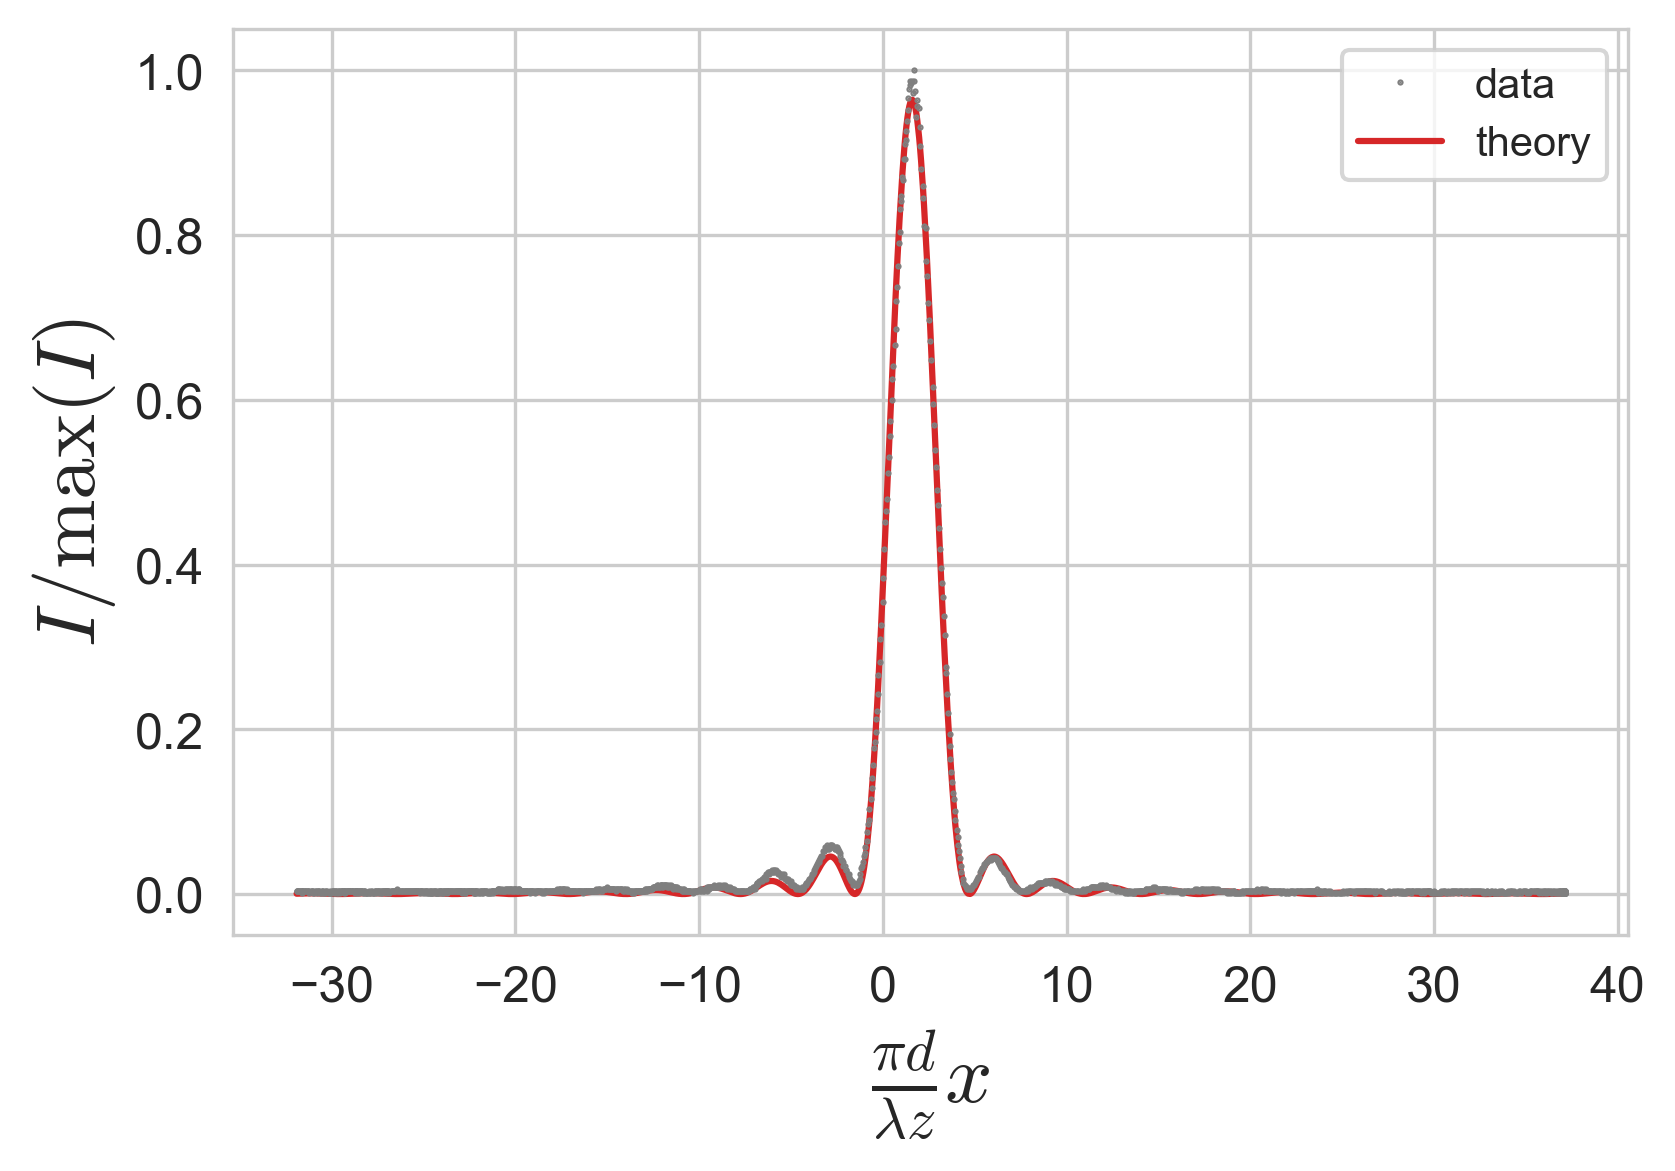
\includegraphics[width=\columnwidth]{figures/single slit interference 0.08mm.png} % first figure itself
		\caption{first figure}
        \label{fig:single slit interference 0.08mm}
	\end{subfigure}\hfill
    \begin{subfigure}{0.5\columnwidth}
        \centering
        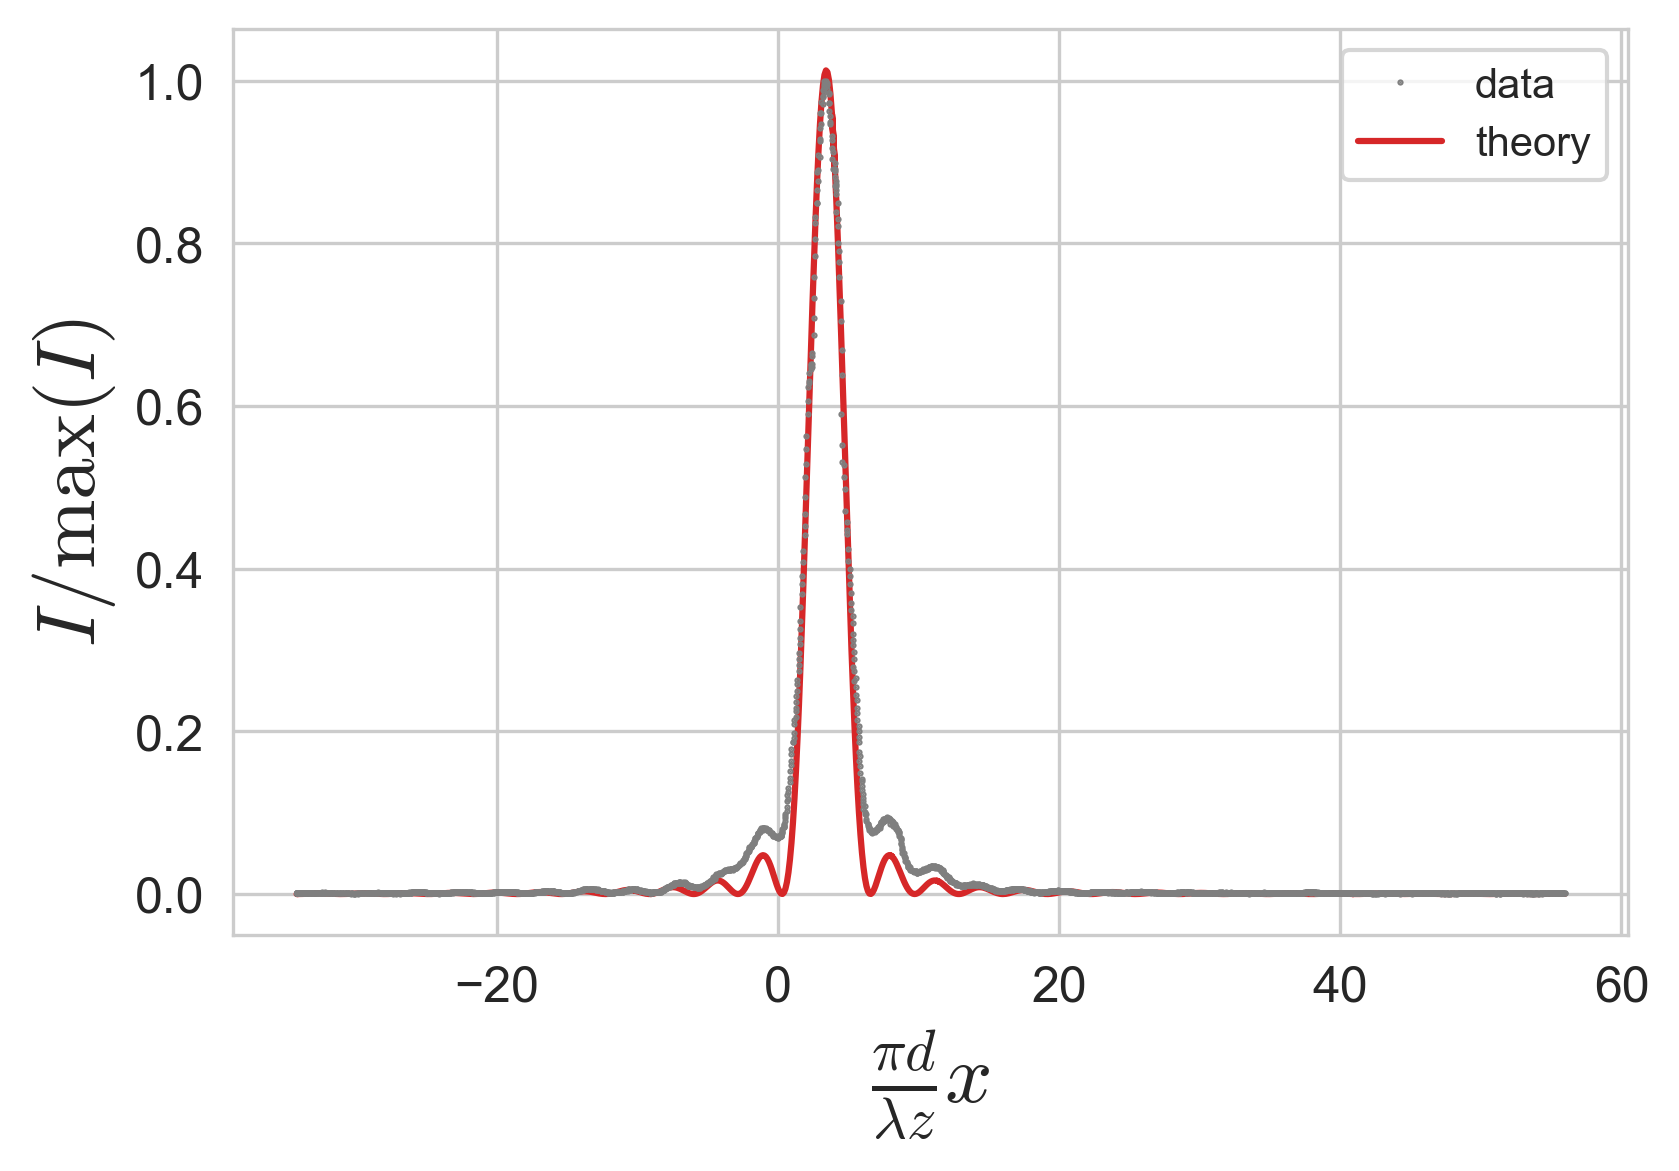
\includegraphics[width=\columnwidth]{figures/single slit interference 0.16mm.png} % second figure itself
        \caption{second figure}
        \label{fig:single slit interference 0.16mm}
    \end{subfigure}
    \label{fig:single slit examples}
\end{figure}

\begin{figure}[H]
    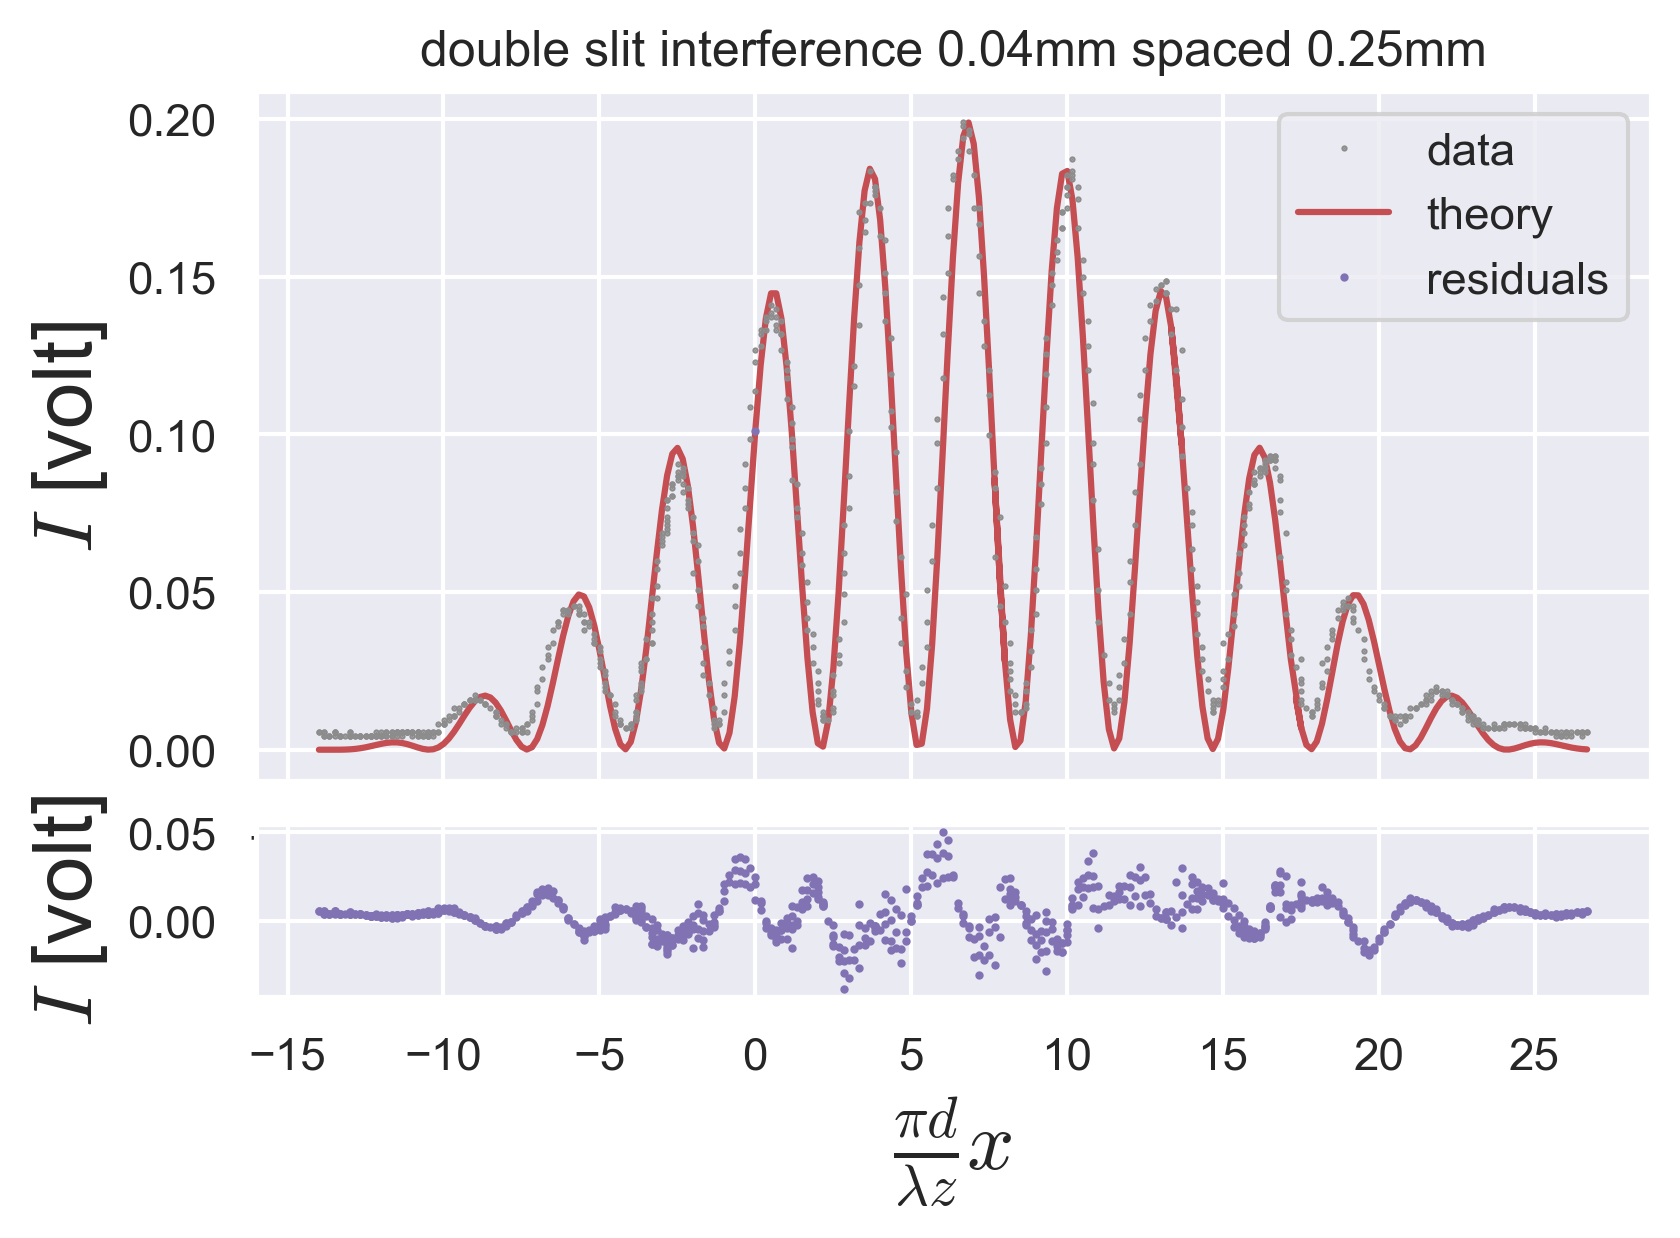
\includegraphics[width=0.9\columnwidth]{figures/0.04w0.25s.png}
    \caption{}
    \label{fig:0.04w0.25s}
\end{figure}
\begin{figure}[H]
    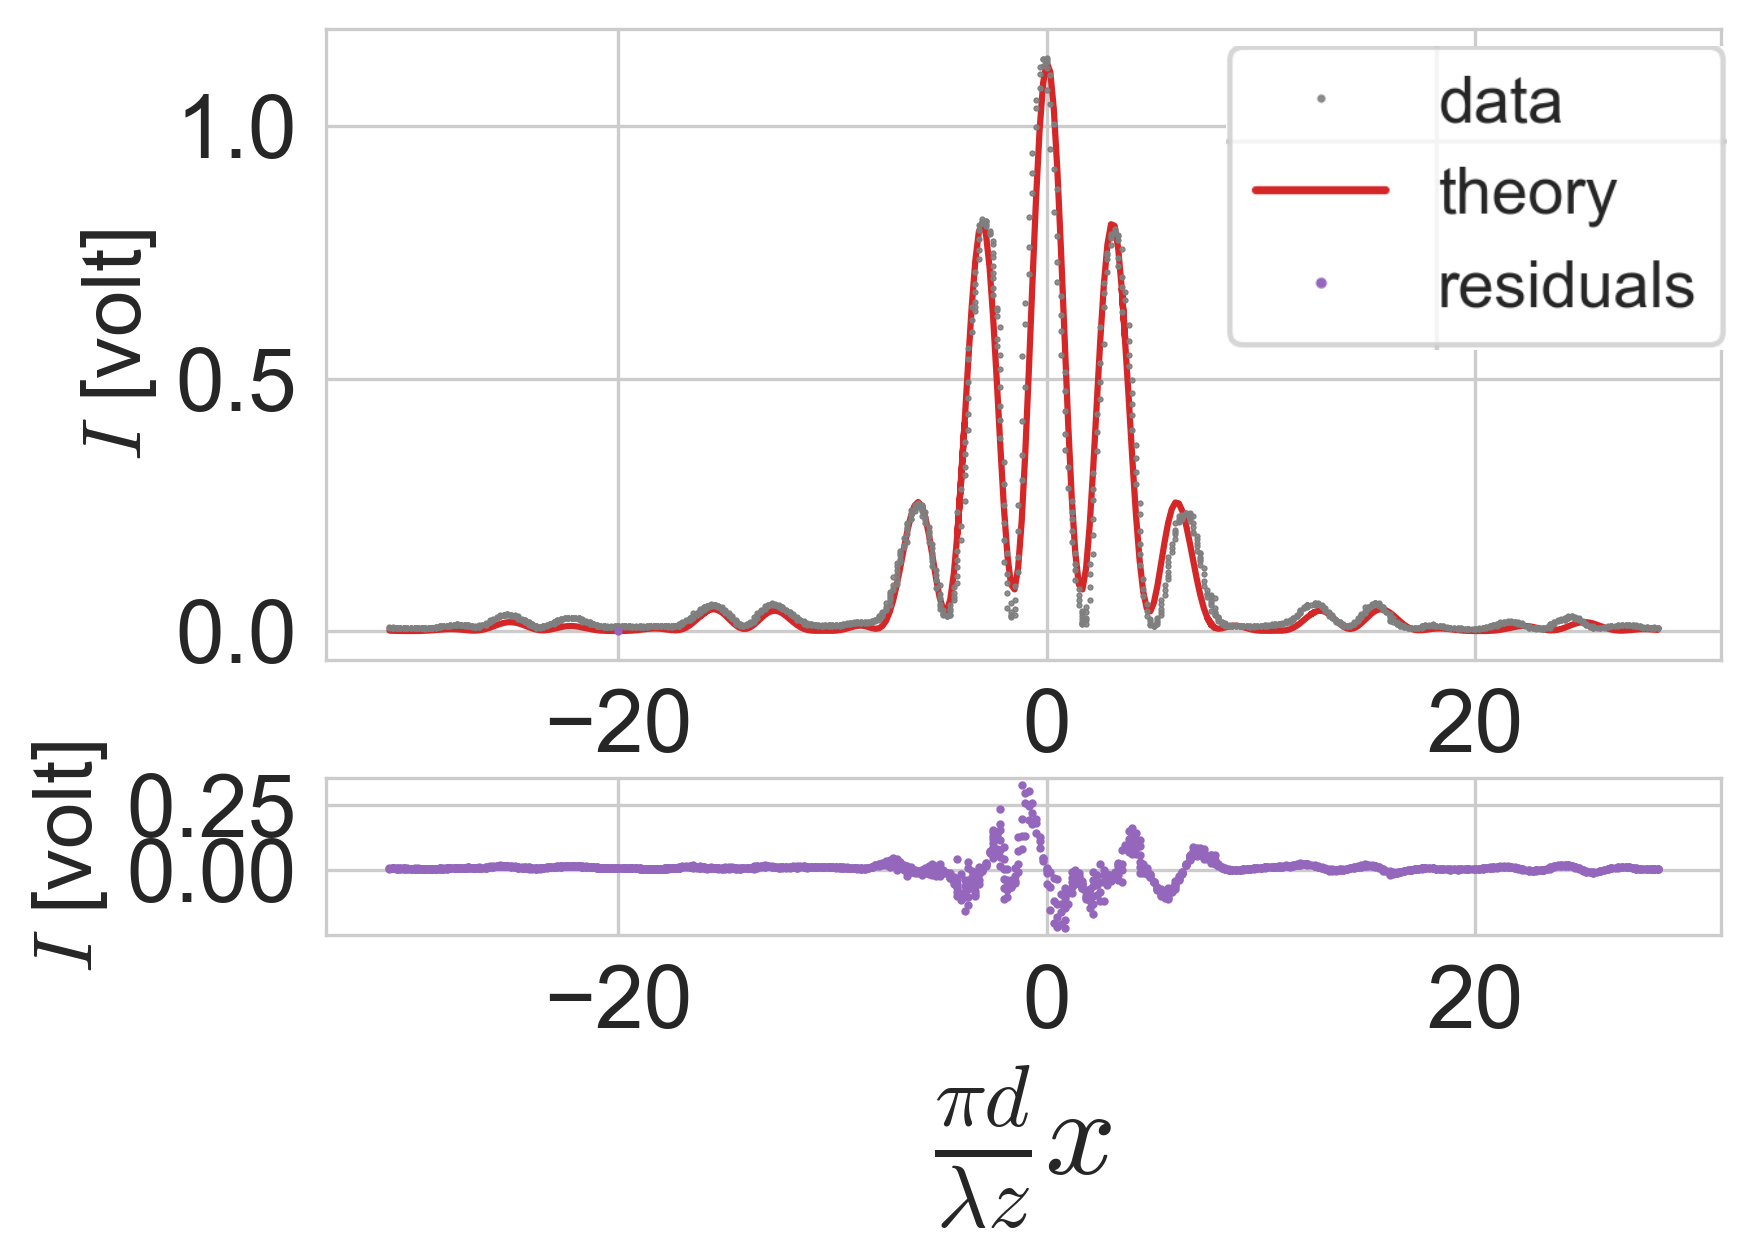
\includegraphics[width=0.9\columnwidth]{figures/0.08w0.25s.png}
    \caption{}
    \label{fig:0.08w0.25s}
\end{figure}
In the case of the periodic diffraction grating "10 lines per mm" the secondary effects are more pronounced especially
the photoelectric sensor's "memory" (The photoelectric sensor has a relaxation period in which to voltage diminishes
therefore after exposure instead of an immediate cut off a slope can be seen as the voltage is recorded with the relation
to the angle which continues to change during said period giving us higher peaks and wider slopes near those peaks)\\
\begin{figure}[H]
    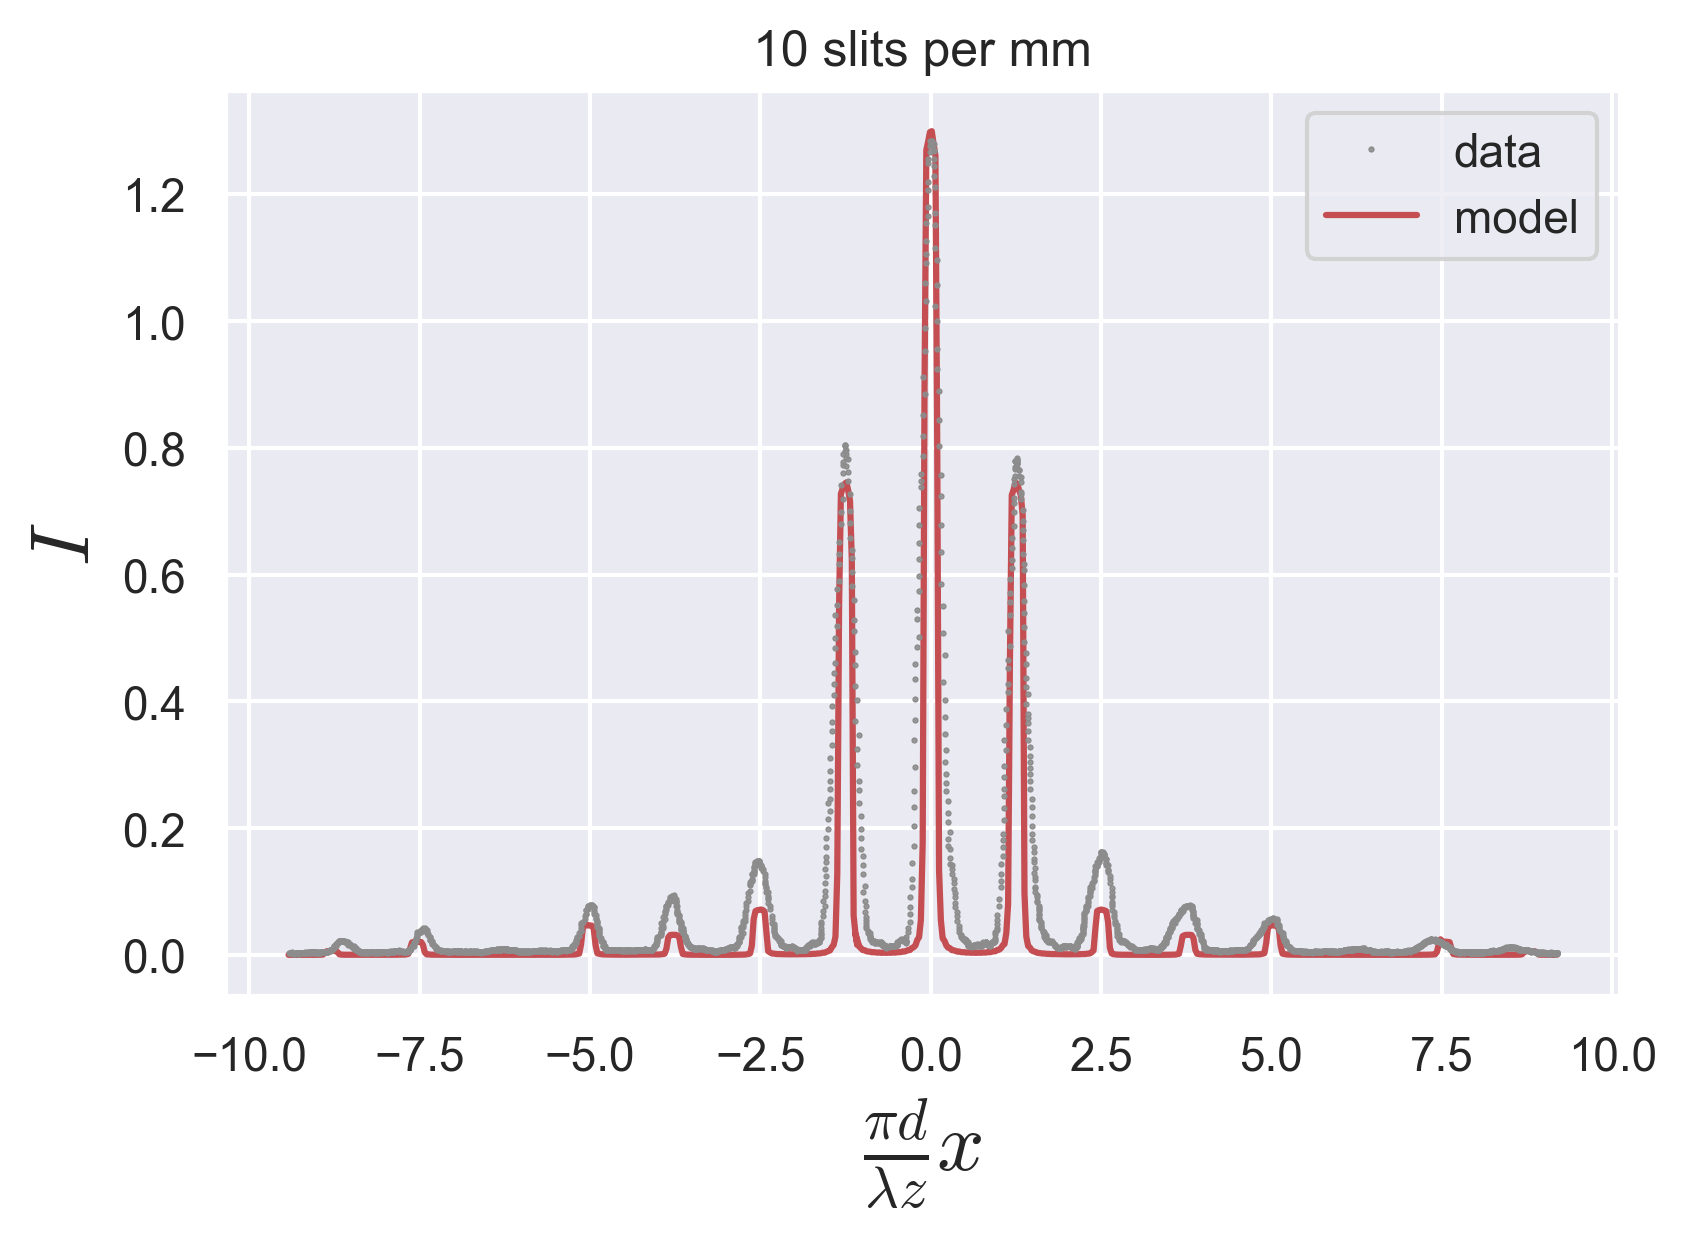
\includegraphics[width=0.9\columnwidth]{figures/10 slits per mm.png}
    \caption{}
    \label{fig:10 slits per mm}
\end{figure}
Finally To justify the title of the paper we should look at the interference pattern of the helix (Which bears some resemblance the shape off DNA)
according to equation (\ref{eqn:farfield}) and the specified approximations the interference pattern can be calculated using
the 2 dimensional fourier transform of the shape of the slit, Taking the inverse fourier transform of the pattern should result
In the square of the shape of the slit (since when calculating the intensity the square of $U$ was taken)
as can be shown by \ref{fig:expansion inverse fourie transform}
\begin{figure}[H]
    \centering
    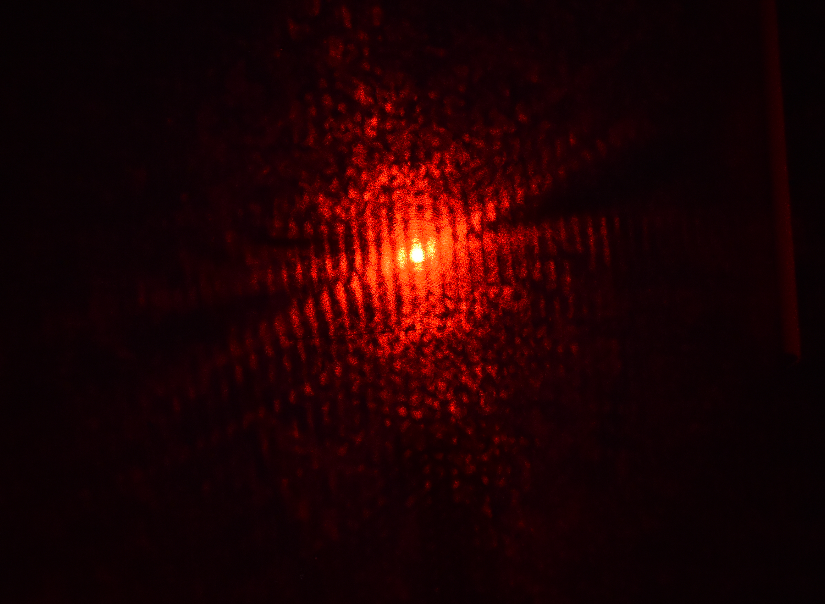
\includegraphics[width=0.9\columnwidth]{figures/expantion meshured interferemce.png}
    \caption{interference pattern measured as a result of diffraction with a helix}
    \label{fig:expansion measured interference pattern}
\end{figure}
\begin{figure}[H]
    \centering
    \begin{subfigure}{0.48\columnwidth}
        \centering
        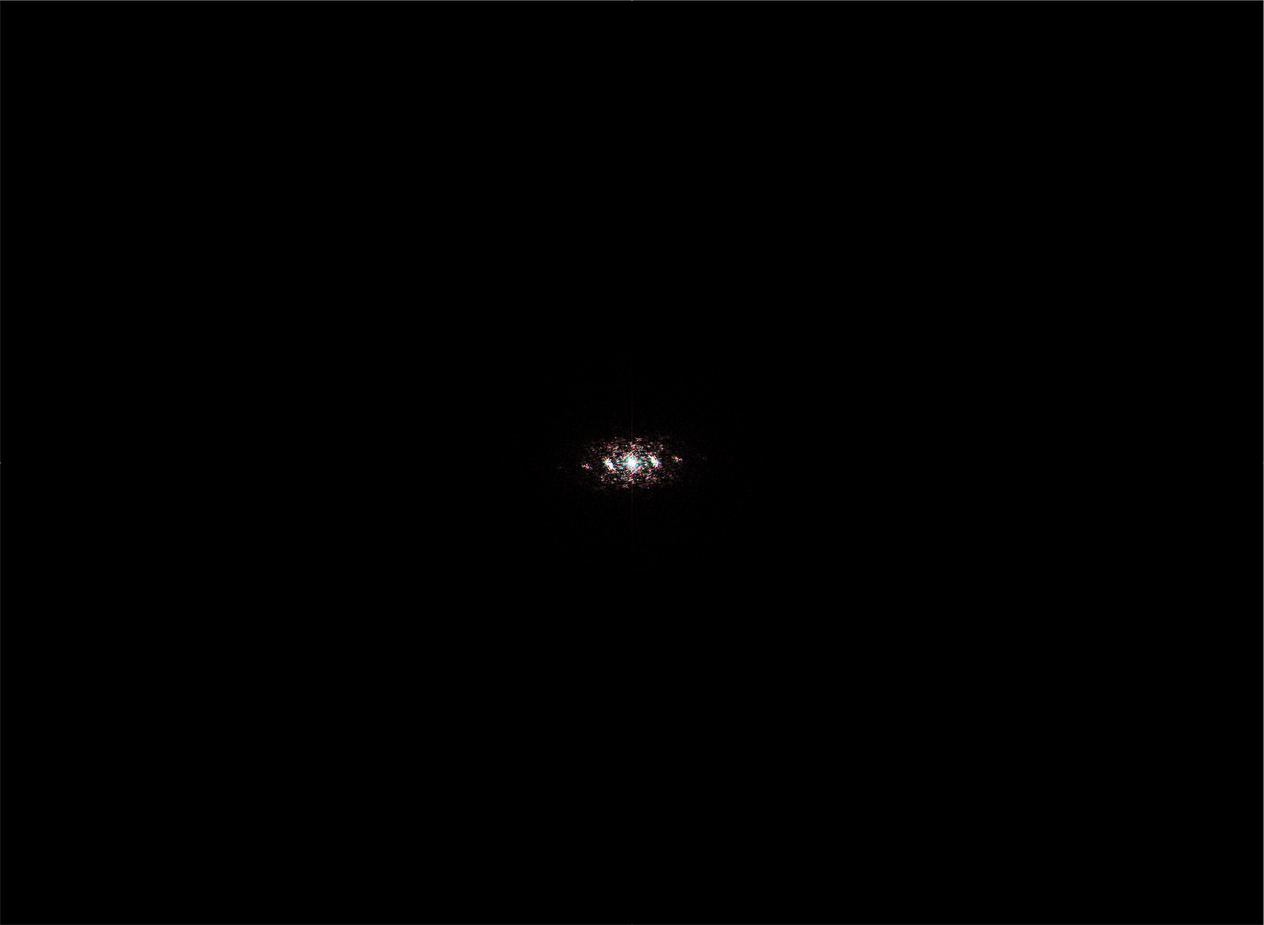
\includegraphics[width=0.9\columnwidth]{figures/expantion fourie transform.png}
        \caption{inverse discrete fourie transform calculated from the interference pattern at of the helix }
        \label{fig:expansion inverse fourie transform measured}
    \end{subfigure}\hfill
    \begin{subfigure}{0.48\columnwidth}
        \centering
        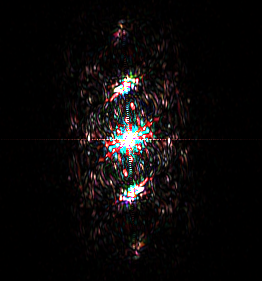
\includegraphics[width=\columnwidth]{figures/expantion fourie transform magnified.png} % second figure itself
        \caption{magnification of\ref{fig:expansion inverse fourie transform measured}}
        \label{fig:expansion fourie transform magnified}
    \end{subfigure}

    \label{fig:expansion theory measurements}
\end{figure}

As can be seen in \ref{fig:expansion fourie transform magnified} The result shows similarity to the calculation done in \ref{fig:expansion inverse fourie transform}
in shape as in the orientation of the spring to the orientation of the "X"